\section{Class}
Class dependence in \G{}.

\tikzstyle{block} = [ellipse, draw, fill=blue!20, text centered]
\tikzstyle{line} = [draw, -latex']

% Markers
\begin{tikzpicture}[node distance =3cm, auto]
    \node [block] (G4VMarker) {G4VMarker};
    \node [block, below of=G4VMarker] (G4Circle) {G4Circle};
    \node [block, left of=G4Circle] (G4Square) {G4Square};
    \node [block, right of=G4Circle] (G4Text) {G4Text};
%    \node [block, above of=G4VMarker] (G4VisAttributes) {G4VisAttributes}; 

    % path
    \path [line] (G4VMarker) -- (G4Circle);
    \path [line] (G4VMarker) -- (G4Square);
    \path [line] (G4VMarker) -- (G4Text);
\end{tikzpicture}

% VsiAttributes
\begin{tikzpicture}[node distance=3cm, auto]
    \node [block] (G4Color) {G4Color};
    \node [block, below of=G4Color] (G4VisAttributes) {G4VisAttributes};
     
    \path [line] (G4Color) -- (G4VisAttributes);
\end{tikzpicture}

\begin{figure}
    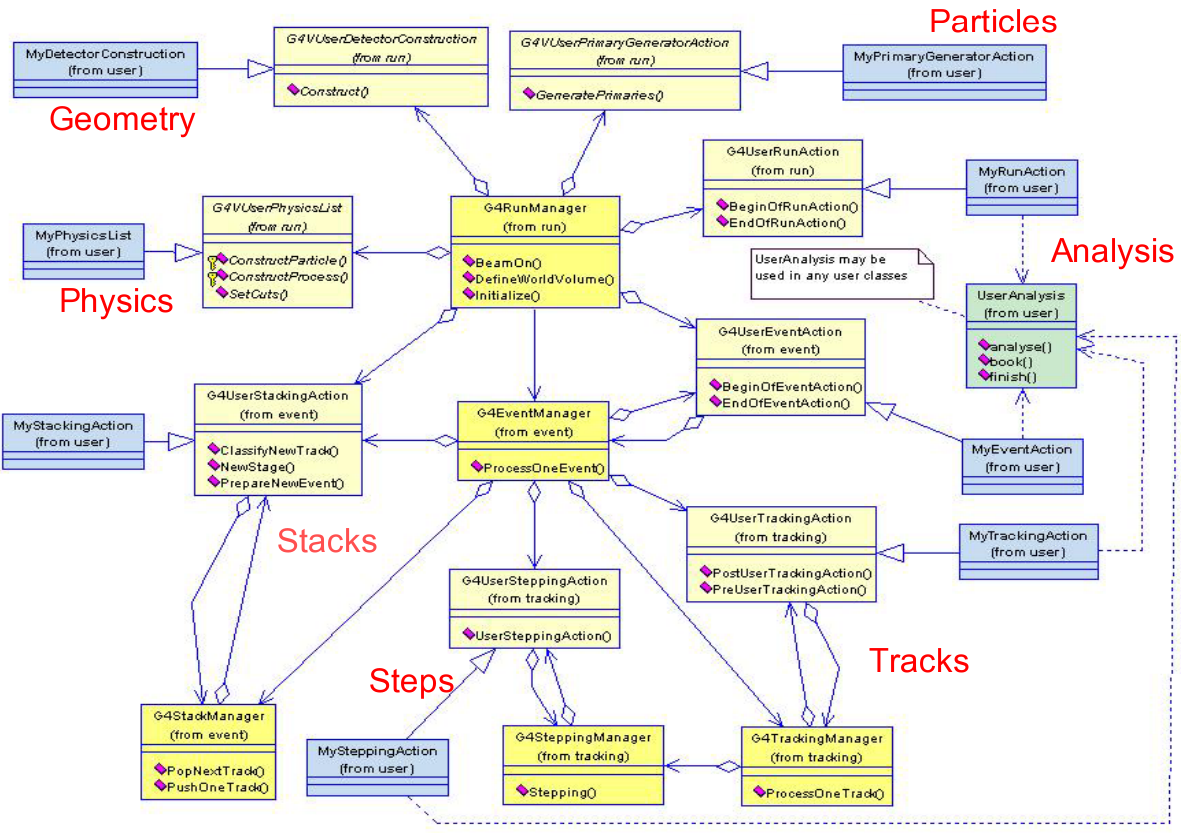
\includegraphics[width=0.9\linewidth]{Geant4_Class.png}
    \caption{Geant4 running example}
    \label{fig_class}
\end{figure}
